\section{Verification of controller}
In this section the 0 \todo{write top}

\subsection{Continuous controller on linear model}
To verify the controller part both of the controllers are first implemented as continuous time controllers in Simulink which can be seen on \autoref{fig:SimulinkControl1}.

\begin{figure}[H]
\centering
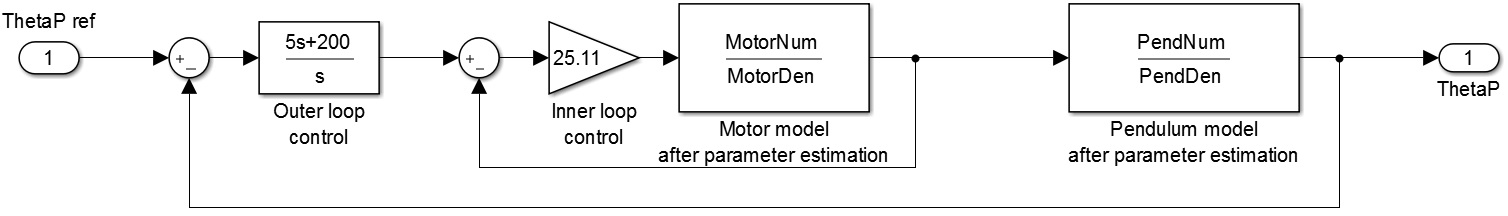
\includegraphics[width = \textwidth]{SimulinkControl1.jpg}
\caption{Simulink implementation of linear model with controller}
\label{fig:SimulinkControl1}
\end{figure}

The system is simulated and a step is applied to the \textit{ThetaP ref}. The results can be seen in \autoref{fig:stepControlSys1}.
\begin{figure}[H]
\centering
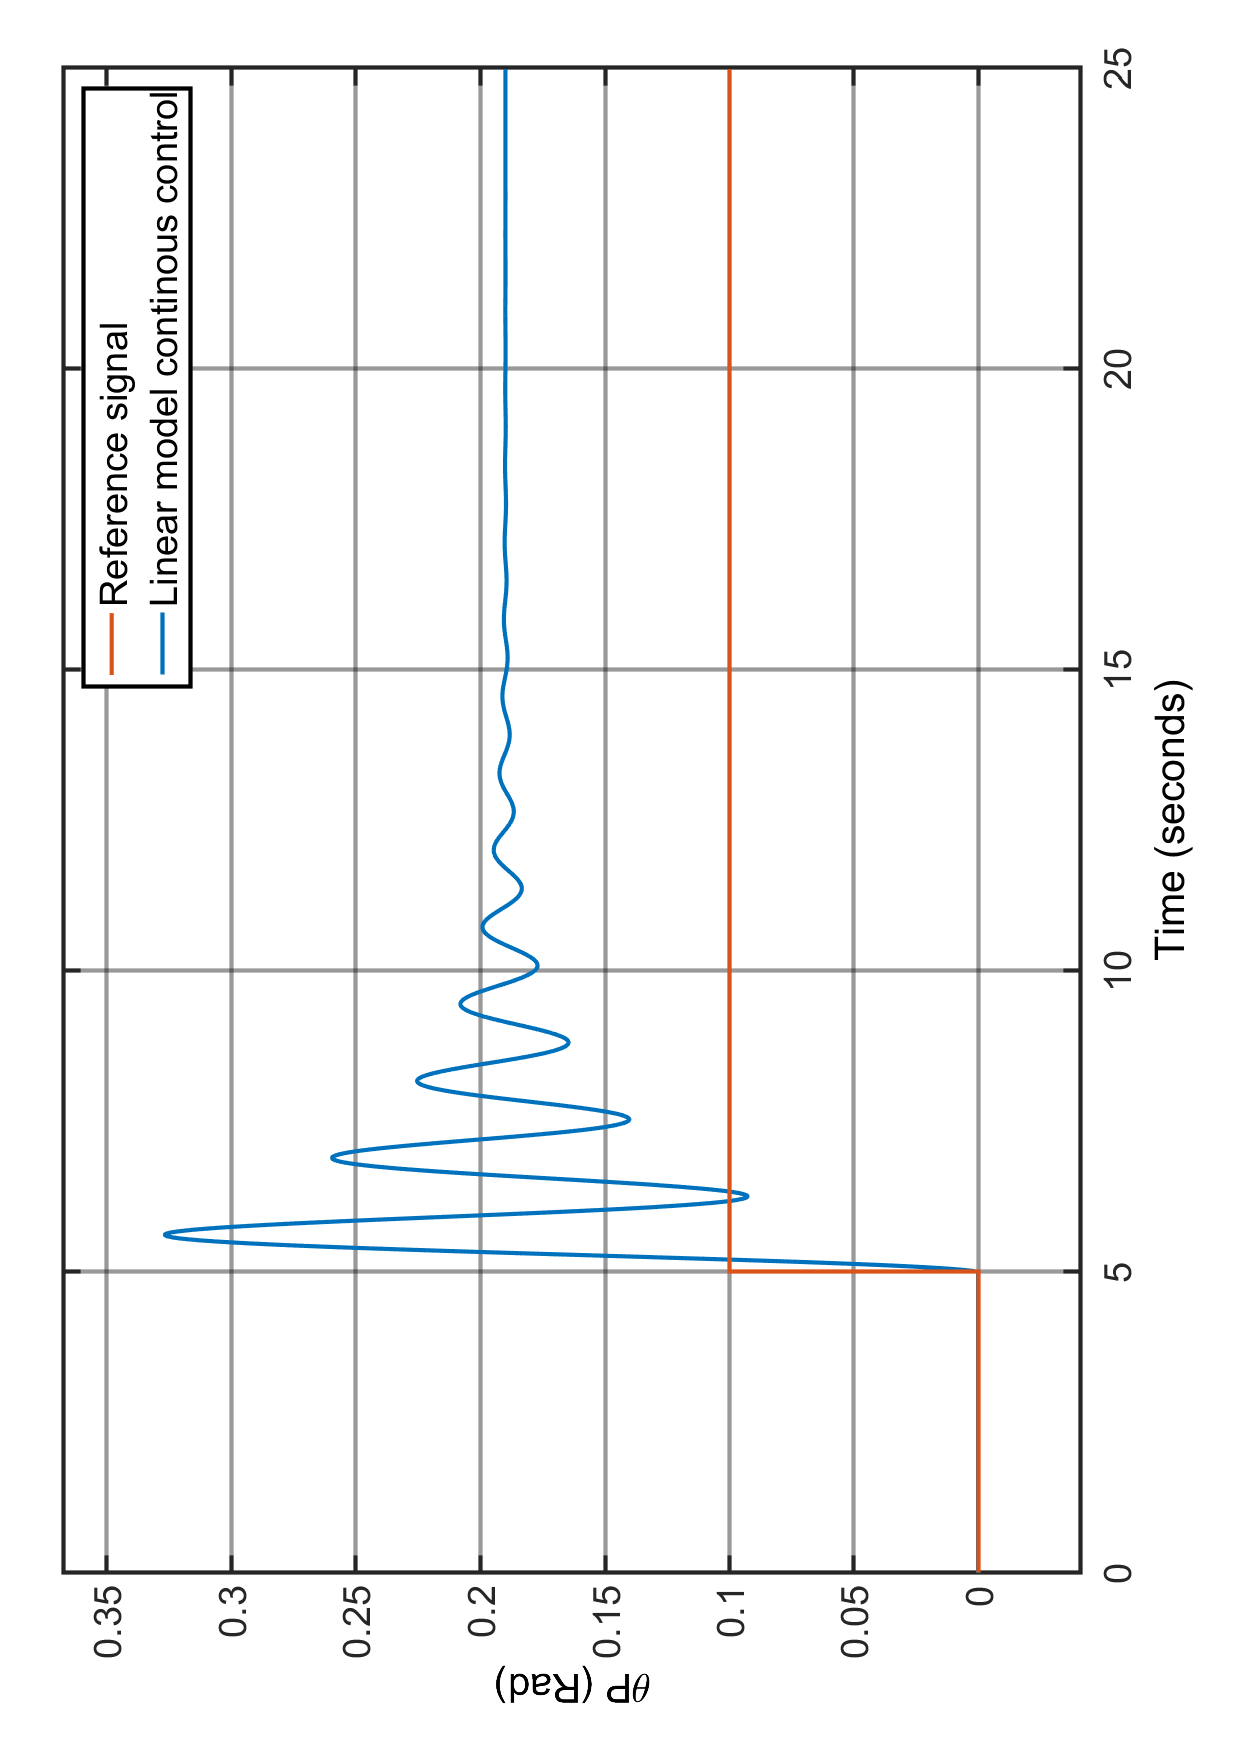
\includegraphics[height = \textwidth, angle = -90]{stepControlSys1.pdf}
\caption{Simulation of linear model with cascade controller.}
\label{fig:stepControlSys1}
\end{figure}

It is seen from the step response that a couple of problems is present in the controller compared to the requirements. First of, the steady state error is quite significant, this problem is ignored due to two reasons. Firstly, a step is not a case the segway should be subjugated to due to the fact that if the segway should be held at a certain angle, it would need to accelerate to infinity which is an unrealistic case. Secondly, time constraints prohibits the option of redesigning the controller. Another problem is, that the settling time, see \autoref{fig:stepControlSys1}, takes approximately ten seconds to settle which is three times longer than the requirement. Also the overshoot is way above the requirement. This would generally require a redesign of the controller, but this is not done due time constraint.
\subsection{Discretized controller on linear model}
Because the continuous time controller is not very good the verification of the discretized controller focus on whether dynamic of the response correlate with that of the continuous time controller, this has also been simulated using Simulink and can be seen in \autoref{fig:stepControlSys2}.
\begin{figure}[H]
\centering
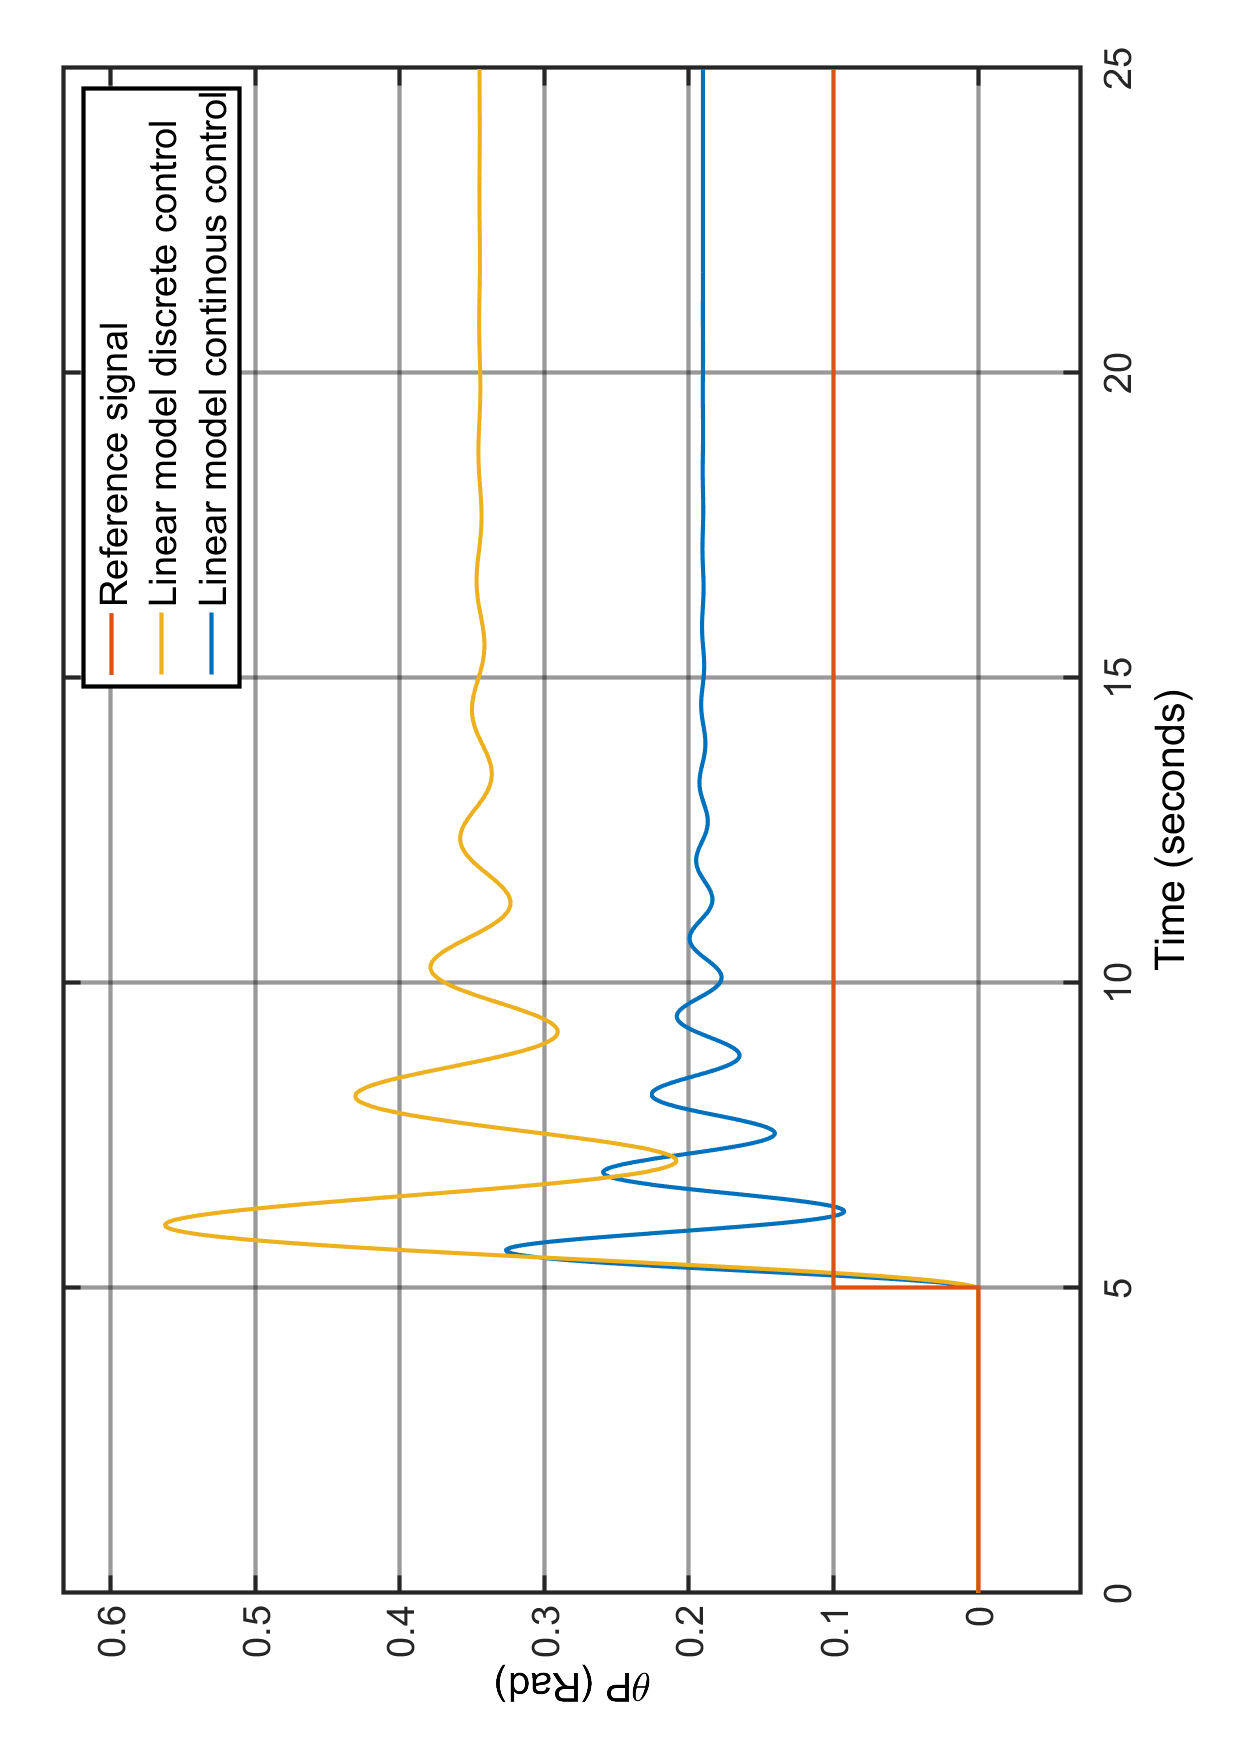
\includegraphics[height = \textwidth, angle = -90]{stepControlSys2.pdf}
\caption{Comparison of simulation of linear model with discretized and continuous controller.}
\label{fig:stepControlSys2}
\end{figure}
From \autoref{fig:stepControlSys2} it can be seen that the settling time of the discretized controller is also around ten seconds and that the overshoot is of a similar magnitude to that of the continuous controller, what differs greatly is however the steady state error, which becomes more than two times greater.  
\subsection{Discretized controller on model}
Finally the discretized controllers are applied to the model, this has also been simulated using Simulink and can be seen in \autoref{fig:stepControlSys3}.
\begin{figure}[H]
\centering
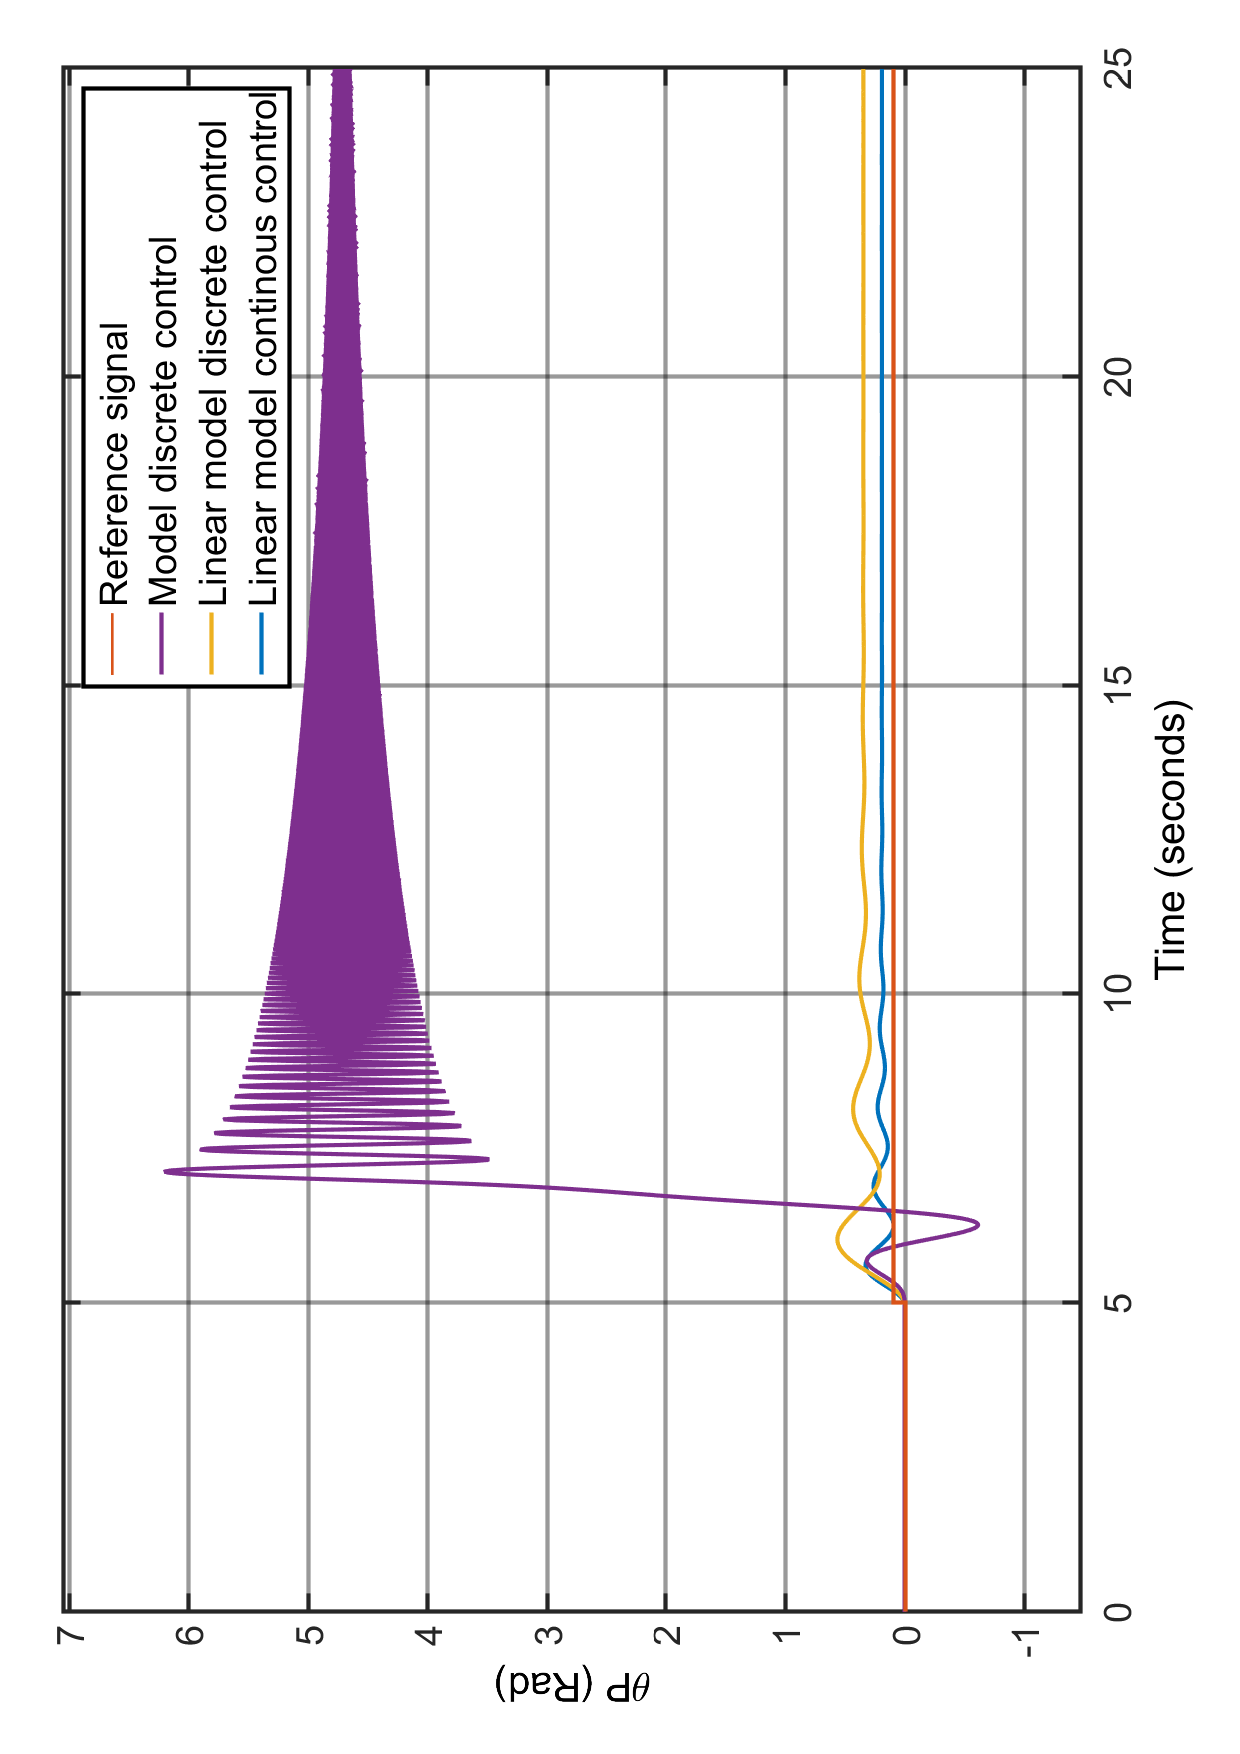
\includegraphics[height = \textwidth, angle = -90]{stepControlSys3.pdf}
\caption{Comparison of simulation of model with discretized controller and linear model with discretized and continuous controller.}
\label{fig:stepControlSys3}
\end{figure}
From \autoref{fig:stepControlSys3} it can be seen that the response changes quite dramatically going from linear model to the derived model. This is not very unexpected as it was already stated that the linerized model deviate from the model more than what could be expected. This is expected to be the reason why the dynamics of the step response changes both in settling time and in cycle time. 
\subsection{Validation}
After implementation of the controllers, it is seen that the segway overreacts to changes and therefore the controller coefficients for the inverted pendulum controller are adjusted and the final filter implementation is 
\begin{equation}
D(z)=\frac{3.8-2.56\cdot z^{-1}}{1-z^{-1}}
\end{equation}
If this controller is applied to the linear model the simulation of a step on the reference result in an unstable response, which can be seen in \autoref{fig:stepControlSys4}, this shows that the model does not describe the reality adequately as expected.
\begin{figure}[H]
\centering
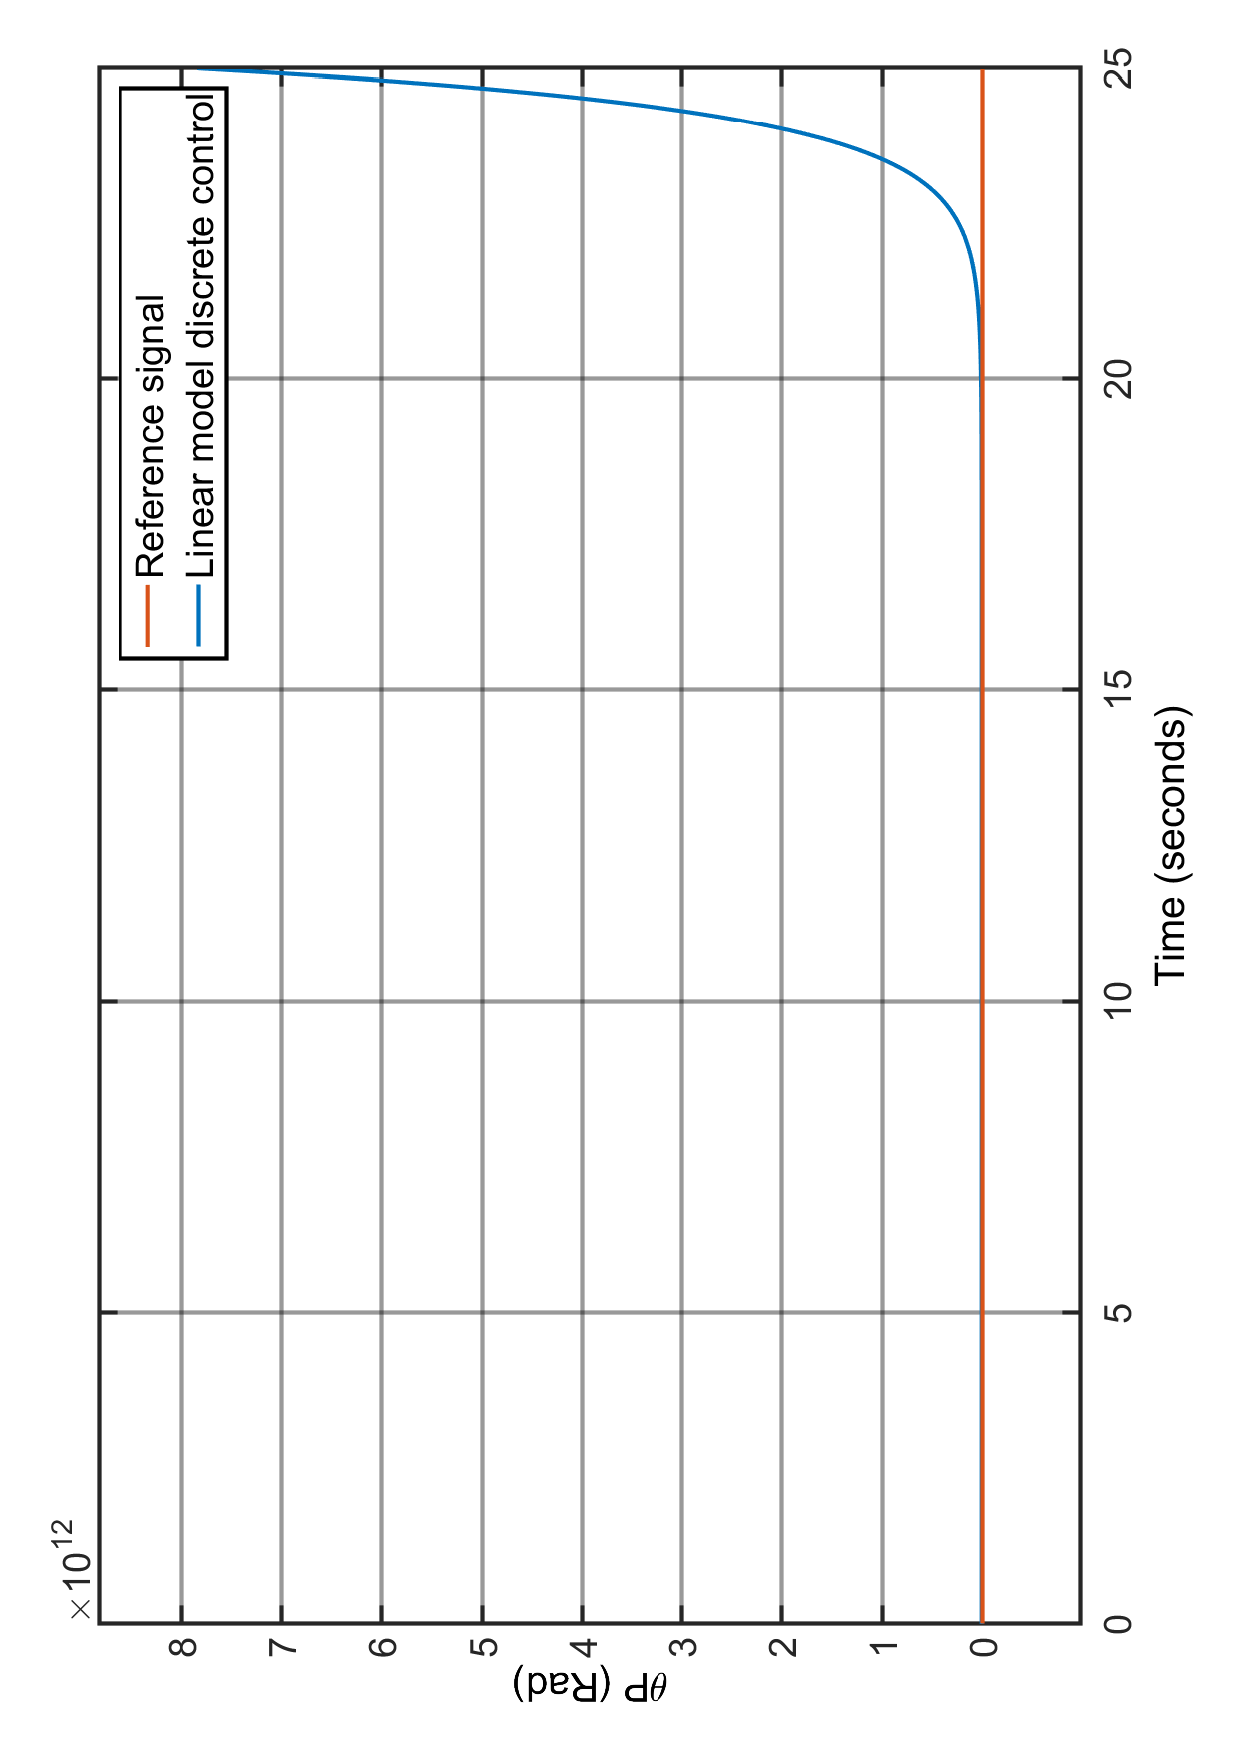
\includegraphics[height = \textwidth, angle = -90]{stepControlSys4.pdf}
\caption{Simulation of implemented controller on linear model.}
\label{fig:stepControlSys4}
\end{figure}
With an implemented controller, the system has turned stable an filters can now be designed to reduce noise from the sensors.